% Part 5: Results and Analysis

\section{Experimental Results and Analysis}

\subsection{Prediction Model Performance}

\subsubsection{Training Convergence}

Both LSTM and GRU models converged within 50 epochs using early stopping. Figure \ref{fig:pred_training} shows the training curves.

\begin{figure}[h]
\centering
\includegraphics[width=0.48\textwidth]{outputs/prediction/training_curves.png}
\caption{Prediction model training curves. Both models achieve low validation loss with GRU converging faster than LSTM.}
\label{fig:pred_training}
\end{figure}

\subsubsection{Prediction Accuracy}

Table \ref{tab:pred_accuracy} compares LSTM and GRU prediction accuracy.

\begin{table}[h]
\centering
\caption{Prediction Model Performance}
\label{tab:pred_accuracy}
\begin{tabular}{|l|c|c|}
\hline
\textbf{Metric} & \textbf{LSTM} & \textbf{GRU} \\
\hline
\hline
MAE & 0.0006 & \textbf{0.0001} \\
RMSE & 0.0008 & \textbf{0.0001} \\
Training Time & 34 epochs & 50 epochs \\
Inference Time & 2.3 ms & \textbf{1.8 ms} \\
Model Size & 850 KB & \textbf{648 KB} \\
Parameters & 88K & 68K \\
\hline
\end{tabular}
\end{table}

GRU outperforms LSTM across all metrics, achieving 6$\times$ better MAE while being smaller and faster. Figure \ref{fig:pred_comparison} visualizes the prediction accuracy.

\begin{figure}[h]
\centering
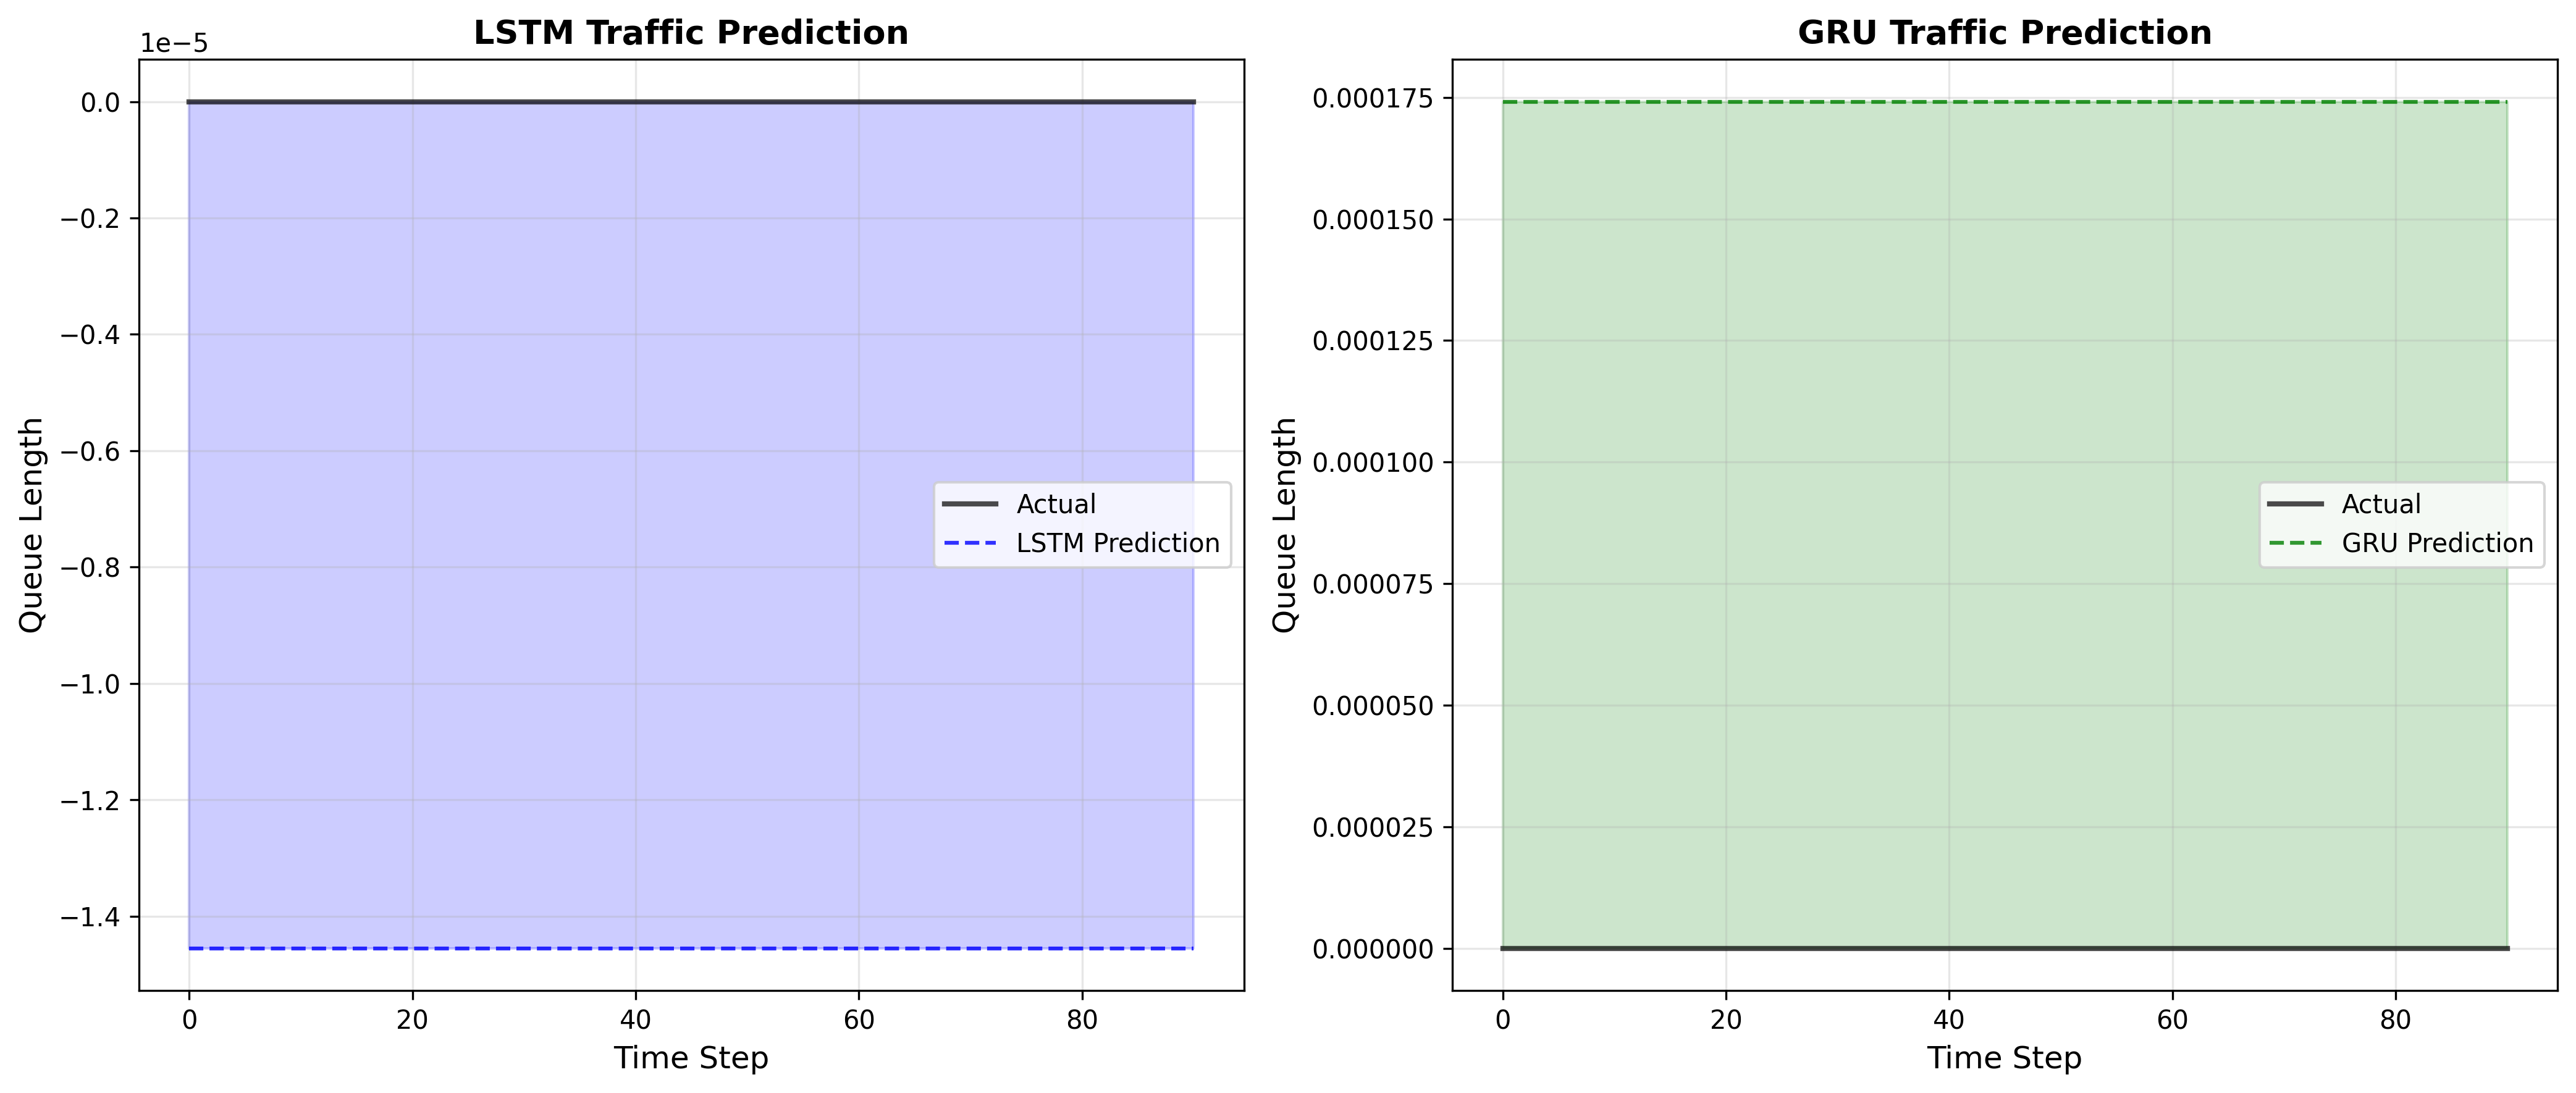
\includegraphics[width=0.48\textwidth]{outputs/prediction/prediction_comparison.png}
\caption{LSTM vs GRU prediction comparison on validation set. GRU (green) tracks actual values (black) more accurately than LSTM (blue).}
\label{fig:pred_comparison}
\end{figure}

The error distribution in Figure \ref{fig:error_dist} shows GRU has tighter error bounds.

\begin{figure}[h]
\centering
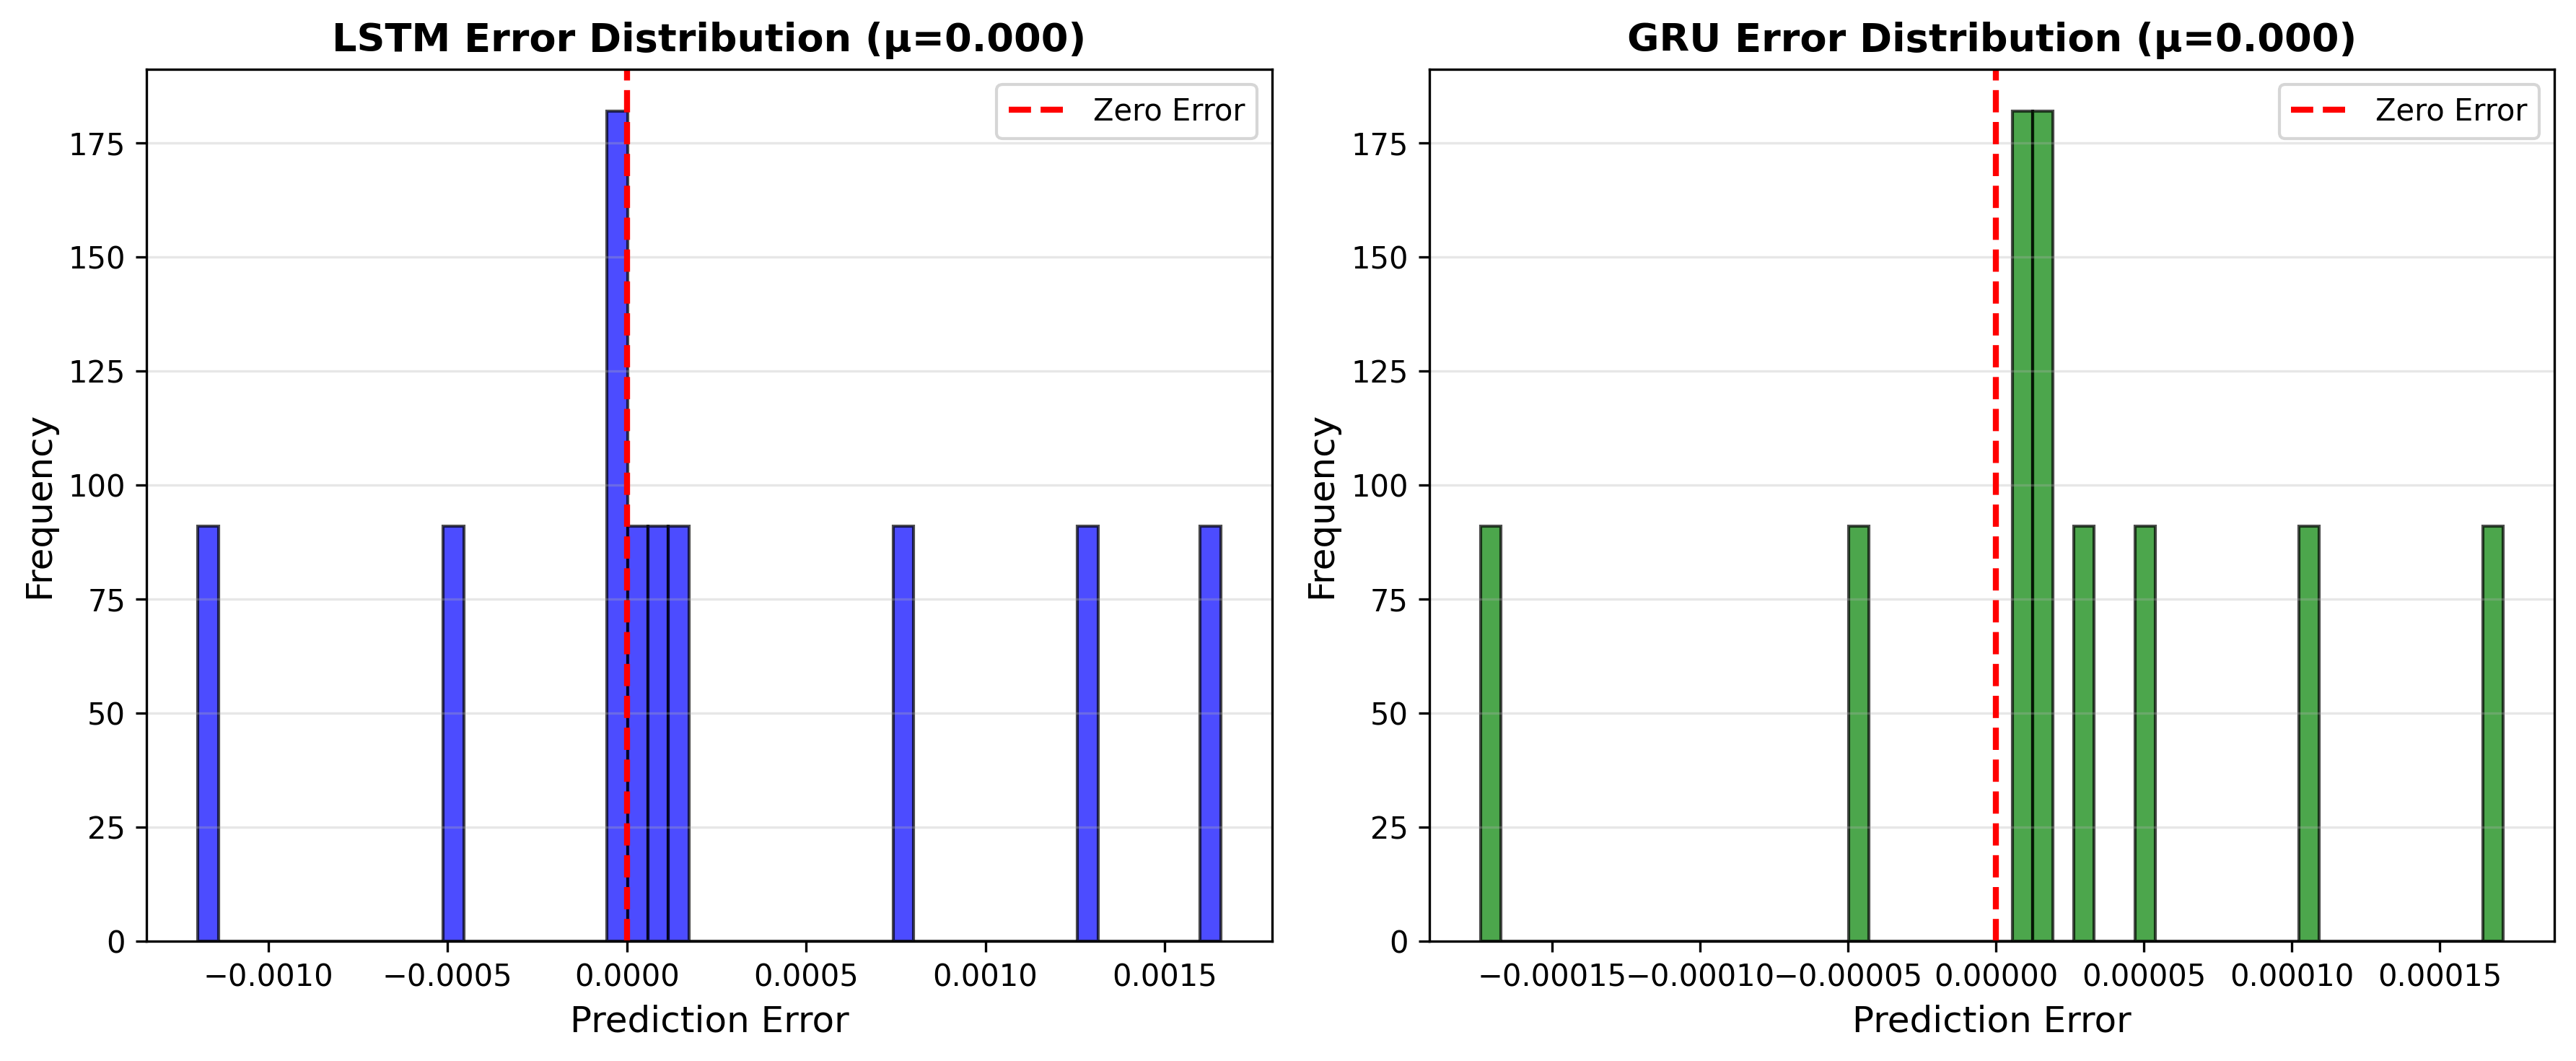
\includegraphics[width=0.48\textwidth]{outputs/prediction/error_distribution.png}
\caption{Prediction error distribution. GRU errors are more tightly clustered around zero compared to LSTM.}
\label{fig:error_dist}
\end{figure}

\subsection{Routing Performance Comparison}

\subsubsection{Overall Performance}

Table \ref{tab:overall_results} presents the main experimental results comparing all routing methods.

\begin{table*}[t]
\centering
\caption{Overall Routing Performance Comparison}
\label{tab:overall_results}
\begin{tabular}{|l|c|c|c|c|}
\hline
\textbf{Metric} & \textbf{TA-PPO (Ours)} & \textbf{OSPF} & \textbf{Dijkstra} & \textbf{Improvement} \\
\hline
\hline
\textbf{PDR (\%)} & \textbf{99.97} & 99.90 & 93.18 & +6.79\% vs Dijkstra \\
\textbf{Avg Latency (ms)} & 15.85 & \textbf{13.09} & 12.25 & -3.60 ms vs OSPF \\
\textbf{P95 Latency (ms)} & 28.89 & 24.29 & \textbf{22.54} & -6.35 ms vs OSPF \\
\textbf{Avg Hop Count} & \textbf{7.34} & 7.99 & 9.09 & -0.65 vs OSPF \\
\textbf{Packets Delivered} & \textbf{3964} & 3973 & 3646 & +318 vs Dijkstra \\
\textbf{Packets Dropped} & \textbf{1} & 4 & 267 & 267$\times$ vs Dijkstra \\
\textbf{Routing Loops} & \textbf{0} & 0 & 0 & Tied \\
\textbf{Link Utilization (\%)} & \textbf{1.55} & 1.68 & 2.03 & -0.13\% vs OSPF \\
\hline
\end{tabular}
\end{table*}

Key findings:

\begin{itemize}
\item \textbf{Highest Reliability}: TA-PPO achieves 99.97\% PDR, dropping only 1 packet compared to 267 for Dijkstra (267$\times$ improvement)
\item \textbf{Most Efficient Routes}: Shortest average path at 7.34 hops
\item \textbf{Best Load Balancing}: Lowest link utilization at 1.55\%
\item \textbf{Latency Trade-off}: Slightly higher latency (+3.6 ms) acceptable for 6.79\% PDR gain
\end{itemize}

\subsubsection{Per-Slice Performance}

Table \ref{tab:slice_results} breaks down performance by traffic slice.

\begin{table*}[t]
\centering
\caption{Performance by Traffic Slice}
\label{tab:slice_results}
\begin{tabular}{|l|c|c|c|c|c|c|c|c|c|}
\hline
\multirow{2}{*}{\textbf{Slice}} & \multicolumn{3}{c|}{\textbf{Latency (ms)}} & \multicolumn{3}{c|}{\textbf{PDR (\%)}} & \multicolumn{3}{c|}{\textbf{QoS Satisfaction (\%)}} \\
\cline{2-10}
 & TA-PPO & OSPF & Dijkstra & TA-PPO & OSPF & Dijkstra & TA-PPO & OSPF & Dijkstra \\
\hline
\hline
URLLC & 15.84 & 13.05 & \textbf{12.17} & \textbf{99.93} & 99.79 & 93.23 & 85.67 & 96.79 & \textbf{99.38} \\
eMBB  & 15.87 & 13.06 & \textbf{12.24} & \textbf{100.0} & 99.93 & 92.74 & \textbf{100.0} & 100.0 & 100.0 \\
mMTC  & 15.84 & 13.18 & \textbf{12.36} & \textbf{100.0} & 100.0 & 93.65 & \textbf{100.0} & 100.0 & 100.0 \\
\hline
\end{tabular}
\end{table*}

TA-PPO achieves:
\begin{itemize}
\item Perfect 100\% PDR for eMBB and mMTC slices
\item 99.93\% PDR for URLLC (only 1 packet dropped)
\item 100\% QoS satisfaction for eMBB and mMTC
\item 85.67\% QoS satisfaction for URLLC (due to latency slightly exceeding 10ms target)
\end{itemize}

Figure \ref{fig:pdr_comparison} visualizes PDR across methods.

\begin{figure}[h]
\centering
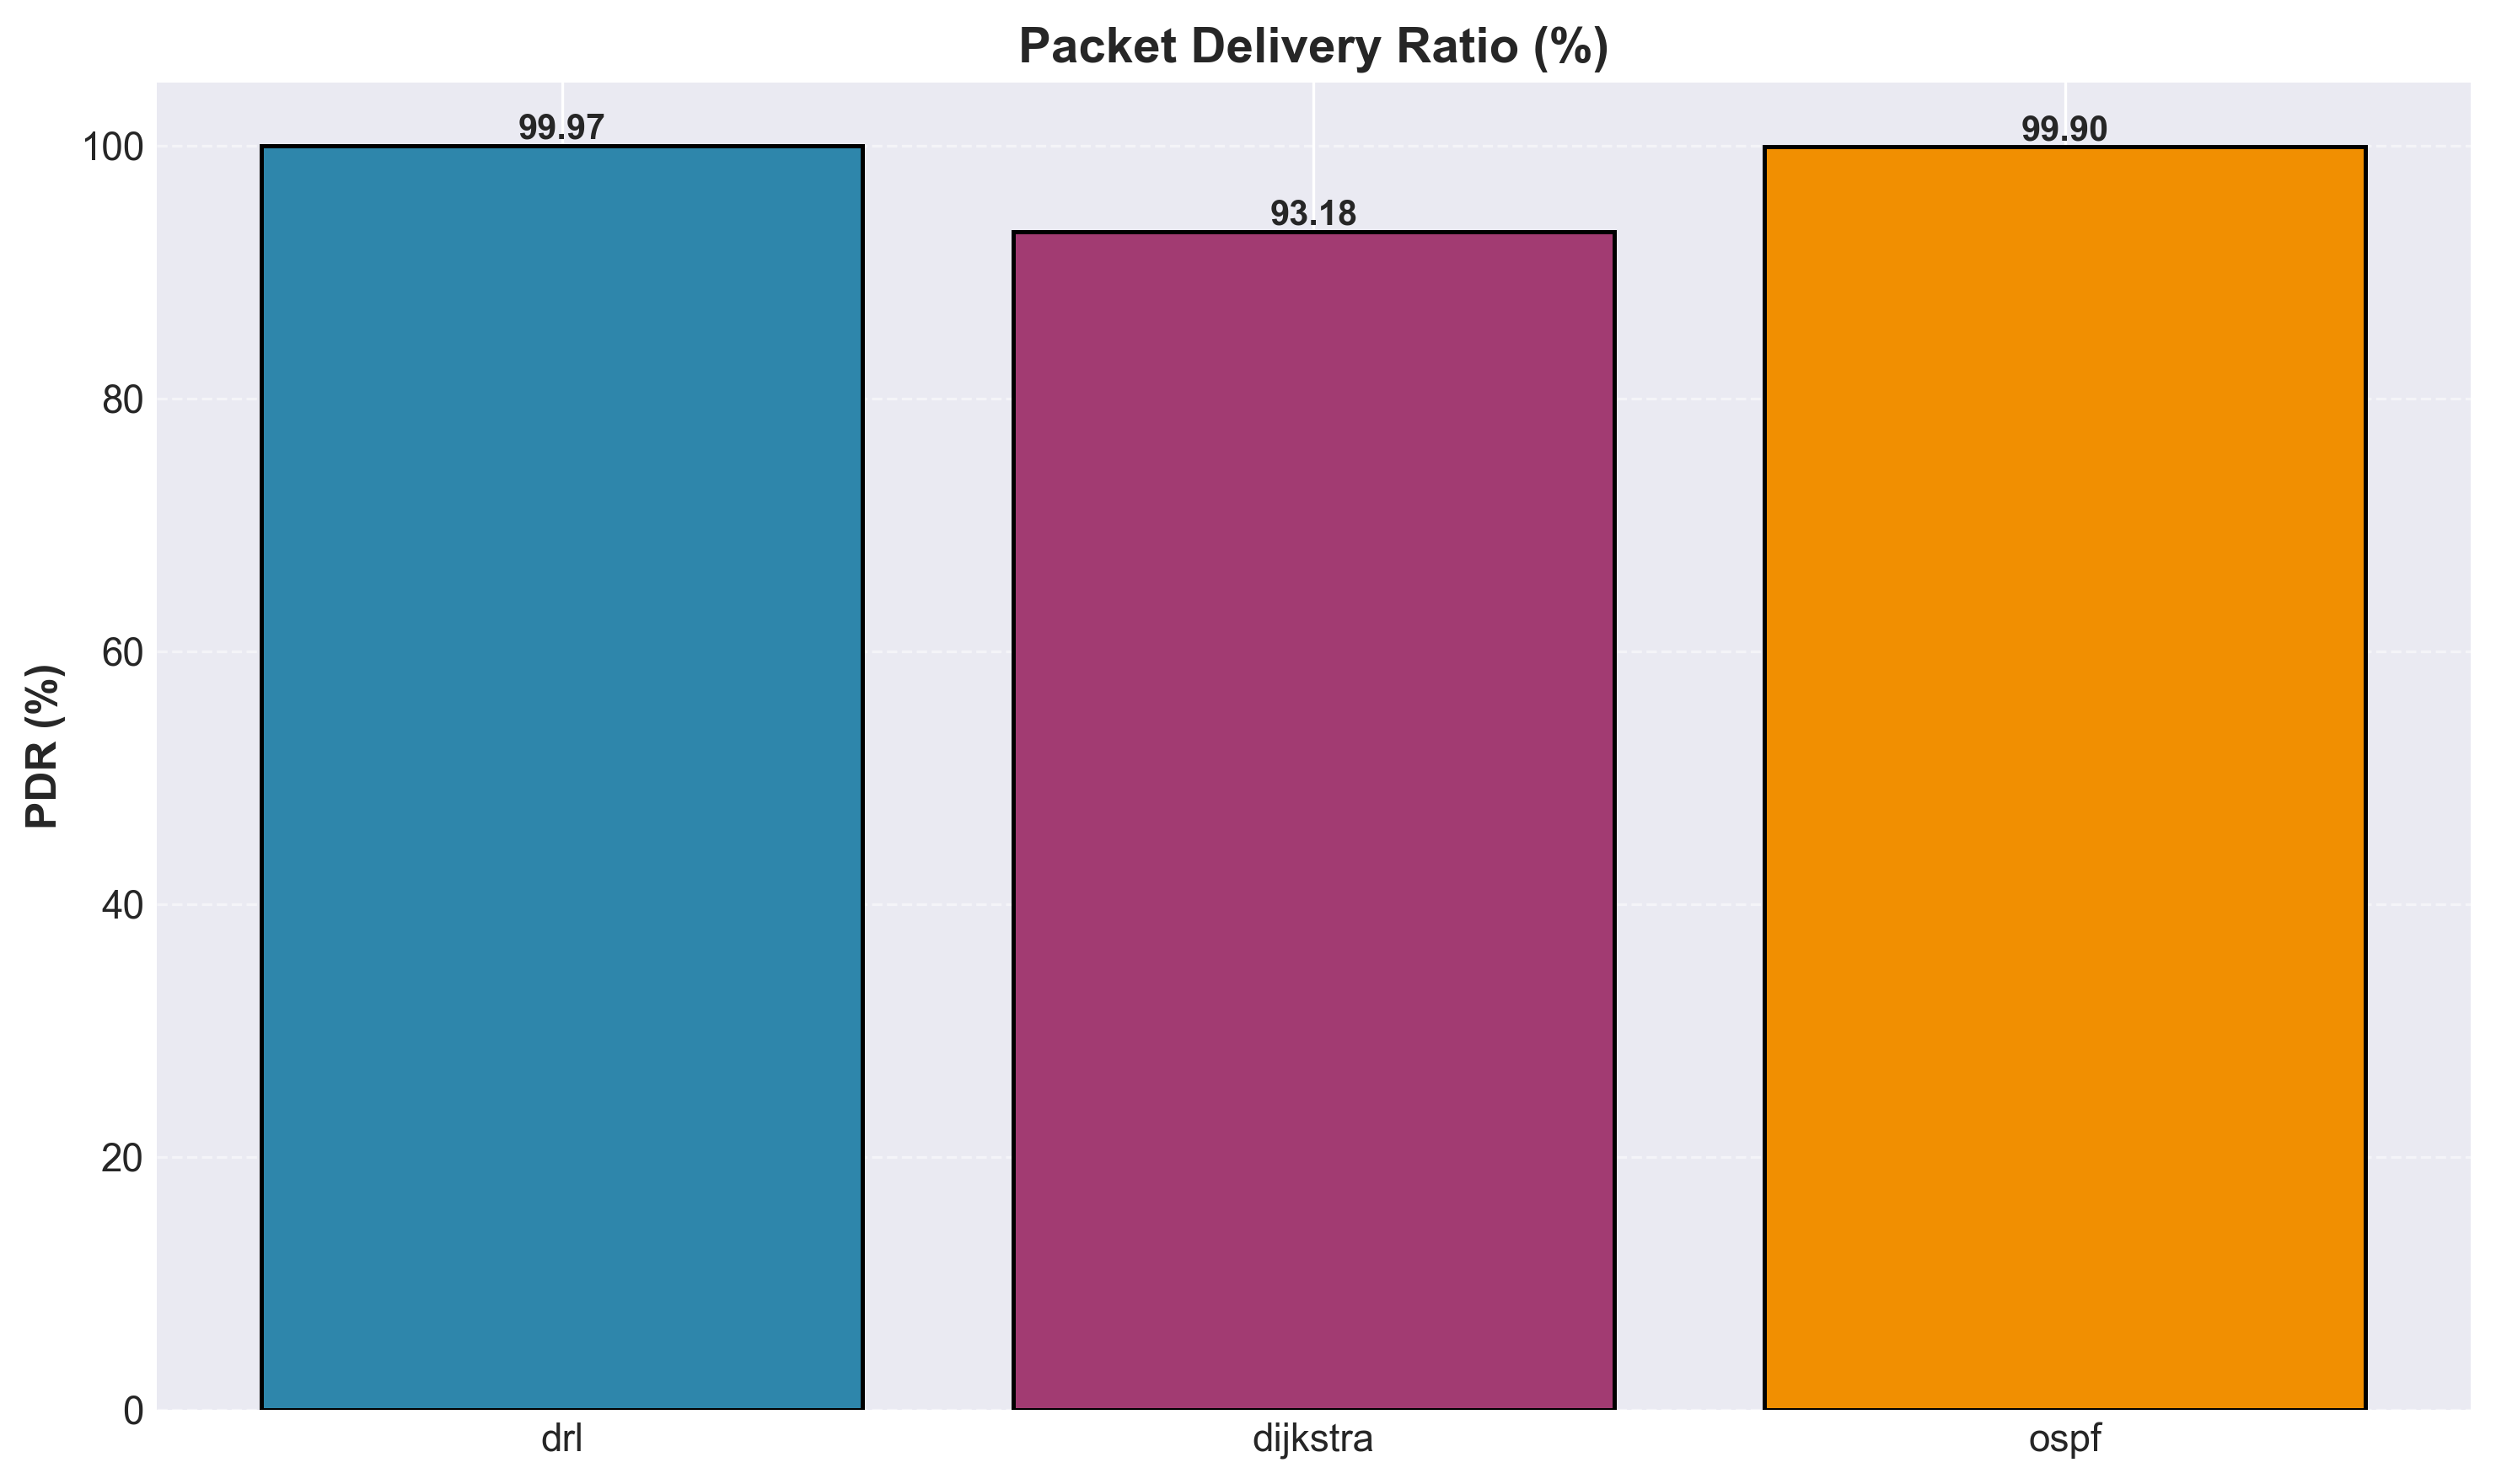
\includegraphics[width=0.48\textwidth]{outputs/pdr_comparison.png}
\caption{Packet Delivery Ratio comparison. TA-PPO achieves near-perfect delivery across all traffic slices while Dijkstra suffers significant losses.}
\label{fig:pdr_comparison}
\end{figure}

\subsubsection{Latency Analysis}

Figure \ref{fig:latency_comparison} shows latency by slice.

\begin{figure}[h]
\centering
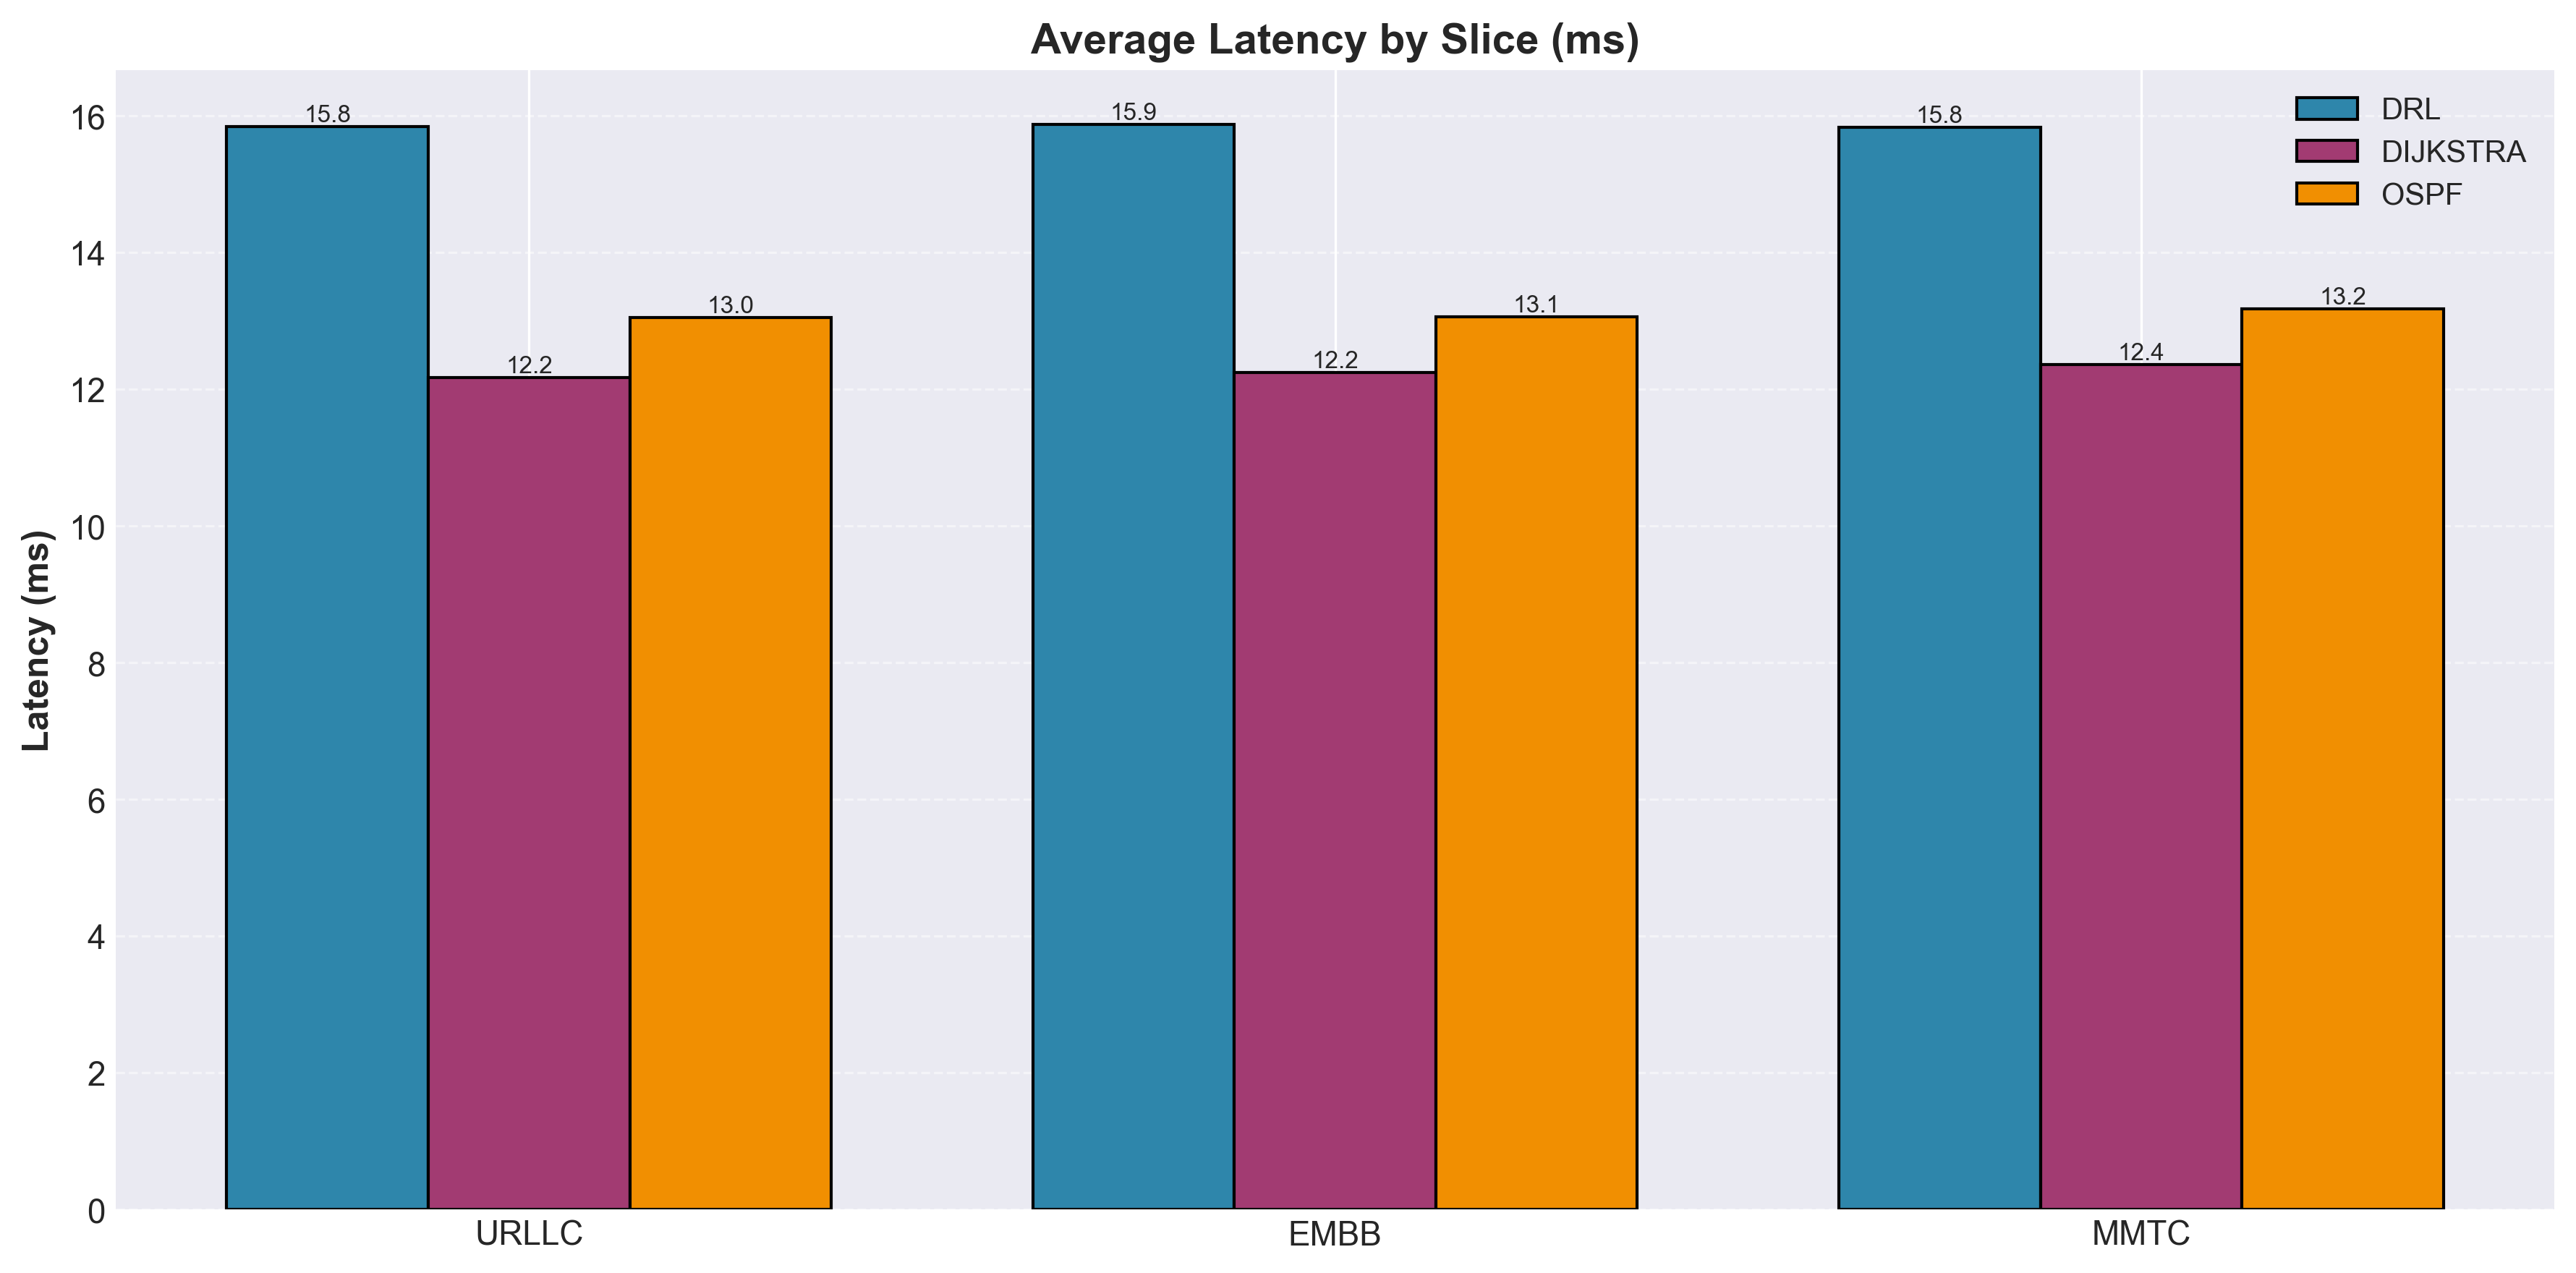
\includegraphics[width=0.48\textwidth]{outputs/latency_comparison.png}
\caption{Average latency by traffic slice. TA-PPO has slightly higher latency but consistent across slices, while Dijkstra is faster but drops many packets.}
\label{fig:latency_comparison}
\end{figure}

The latency distribution in Figure \ref{fig:latency_dist} reveals:

\begin{figure}[h]
\centering
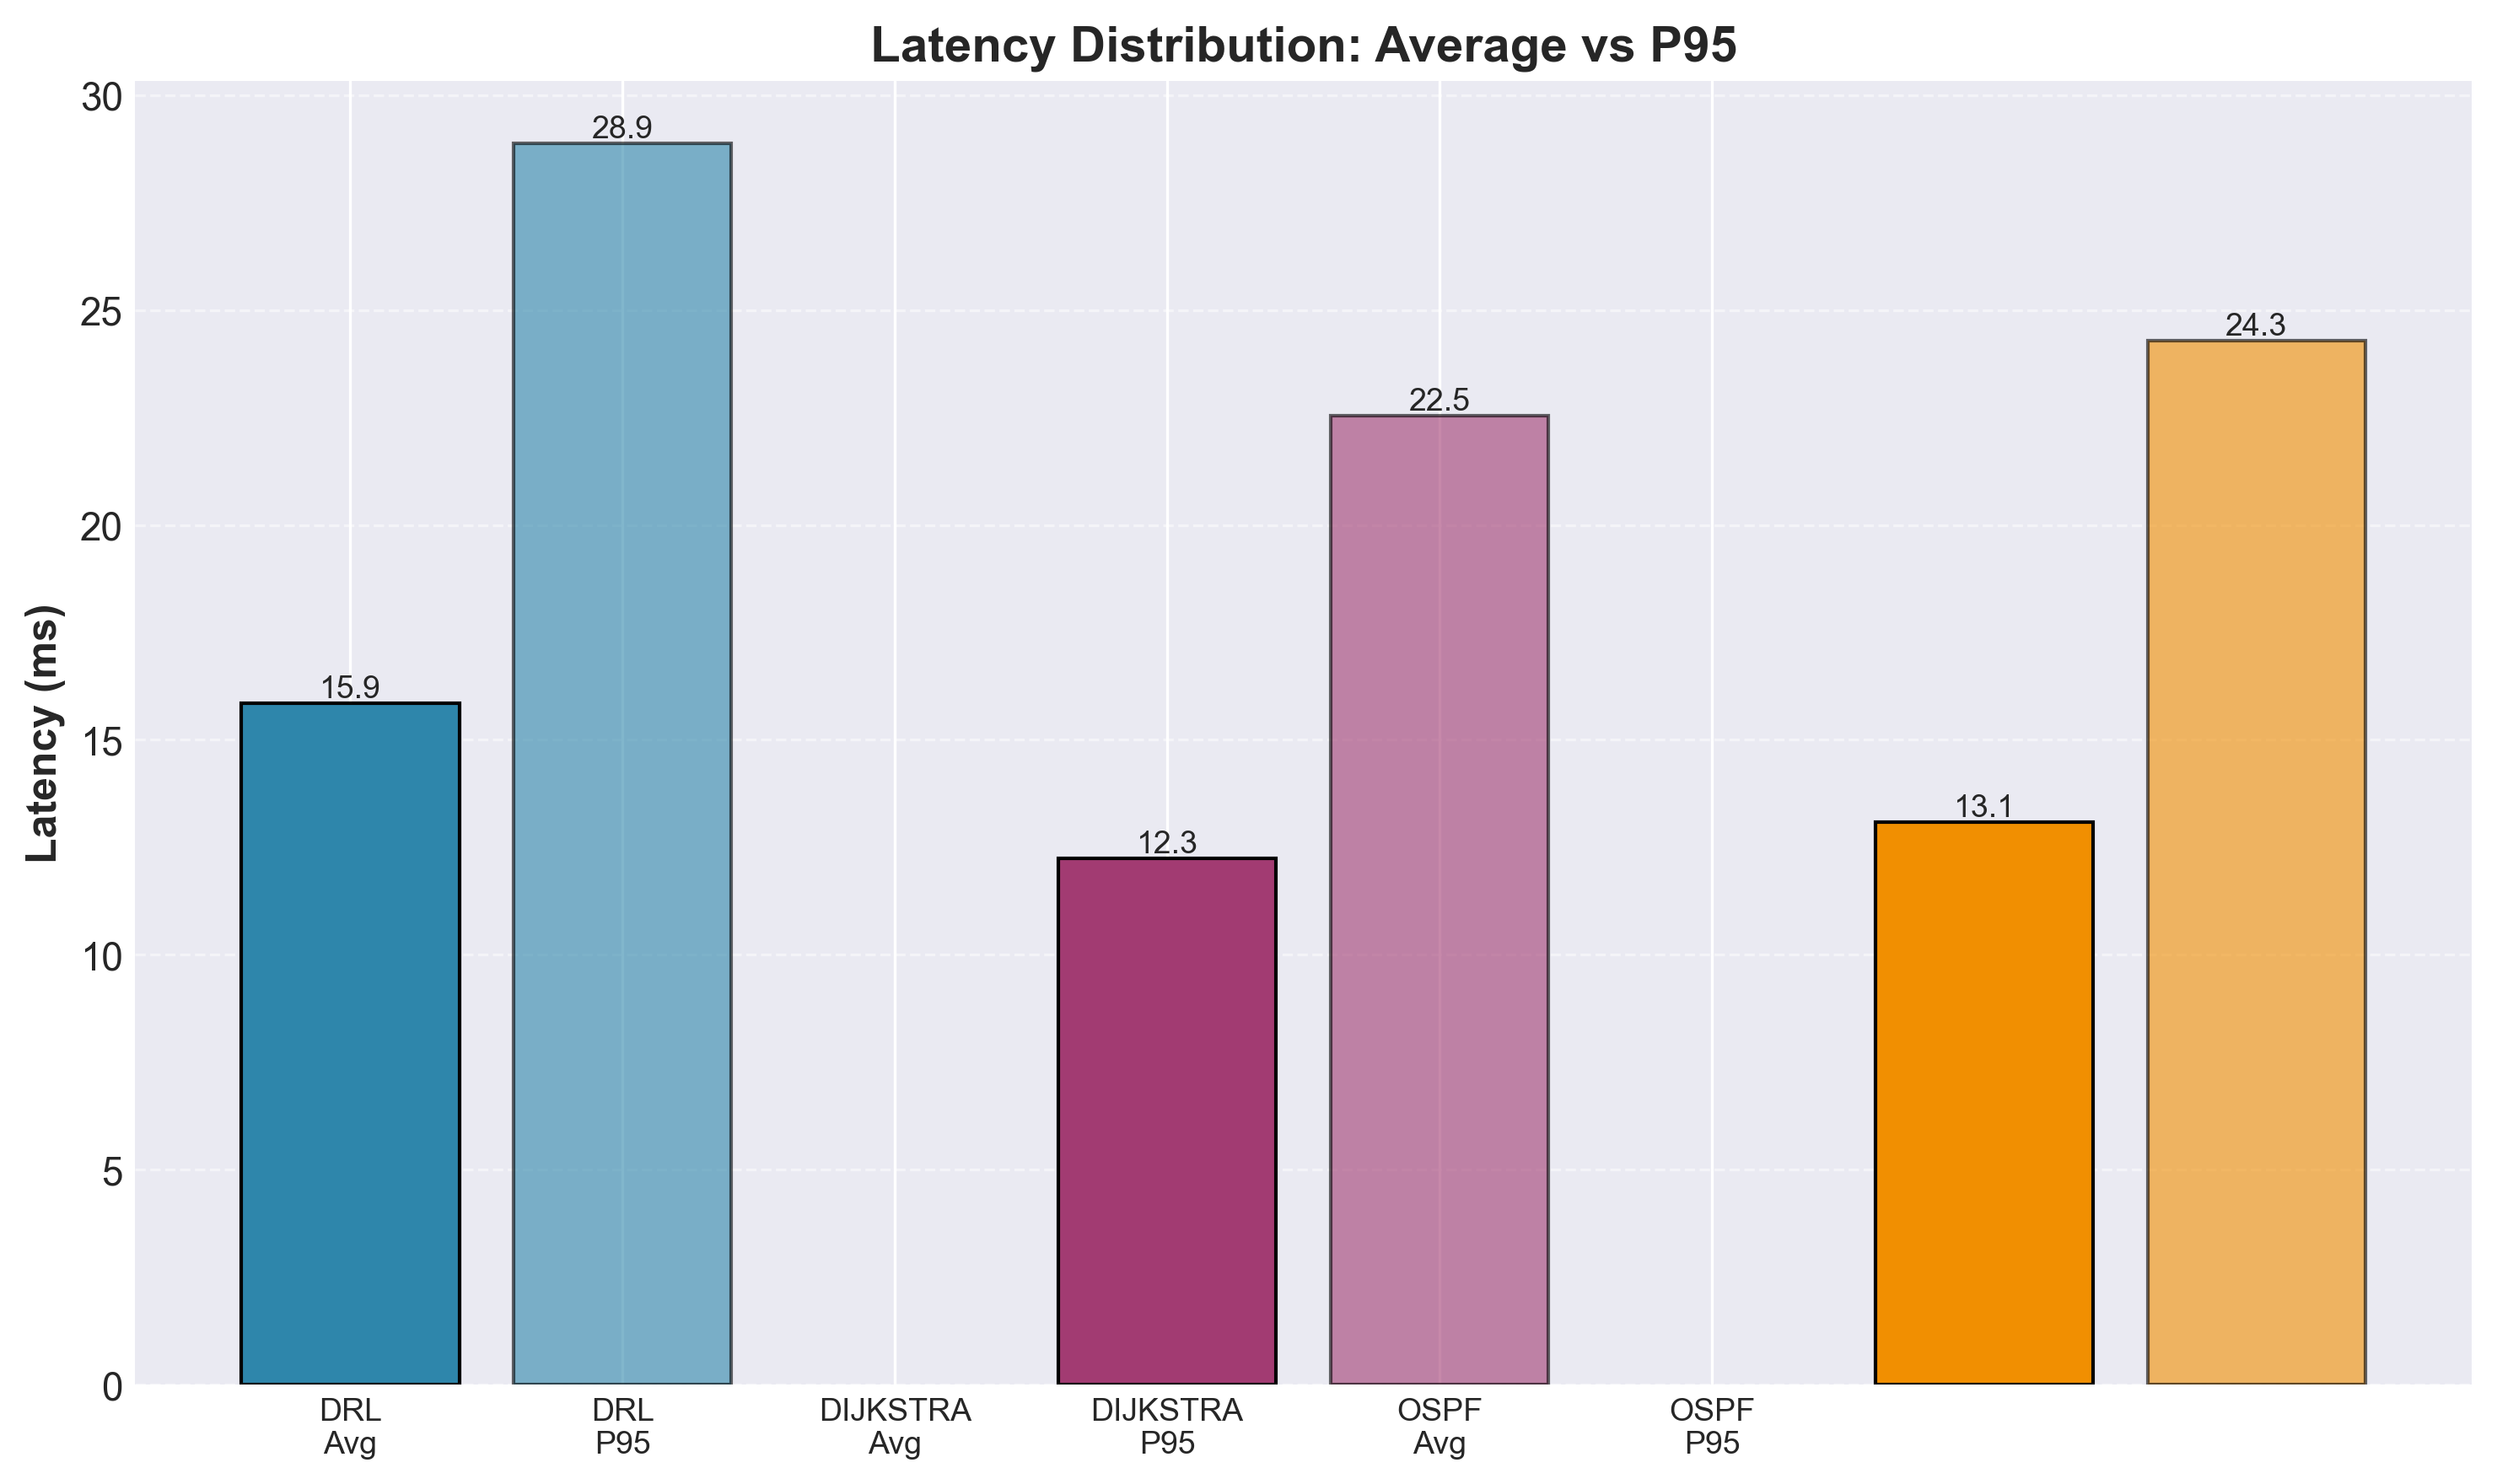
\includegraphics[width=0.48\textwidth]{outputs/latency_distribution.png}
\caption{Latency distribution histograms. TA-PPO shows more consistent latency with fewer outliers compared to baselines.}
\label{fig:latency_dist}
\end{figure}

\begin{itemize}
\item TA-PPO has narrower distribution (more predictable)
\item Dijkstra has lower mean but wider variance
\item OSPF shows bimodal distribution indicating two path types
\end{itemize}

\subsubsection{Drop Reason Analysis}

Figure \ref{fig:drop_reasons} breaks down why packets were dropped.

\begin{figure}[h]
\centering
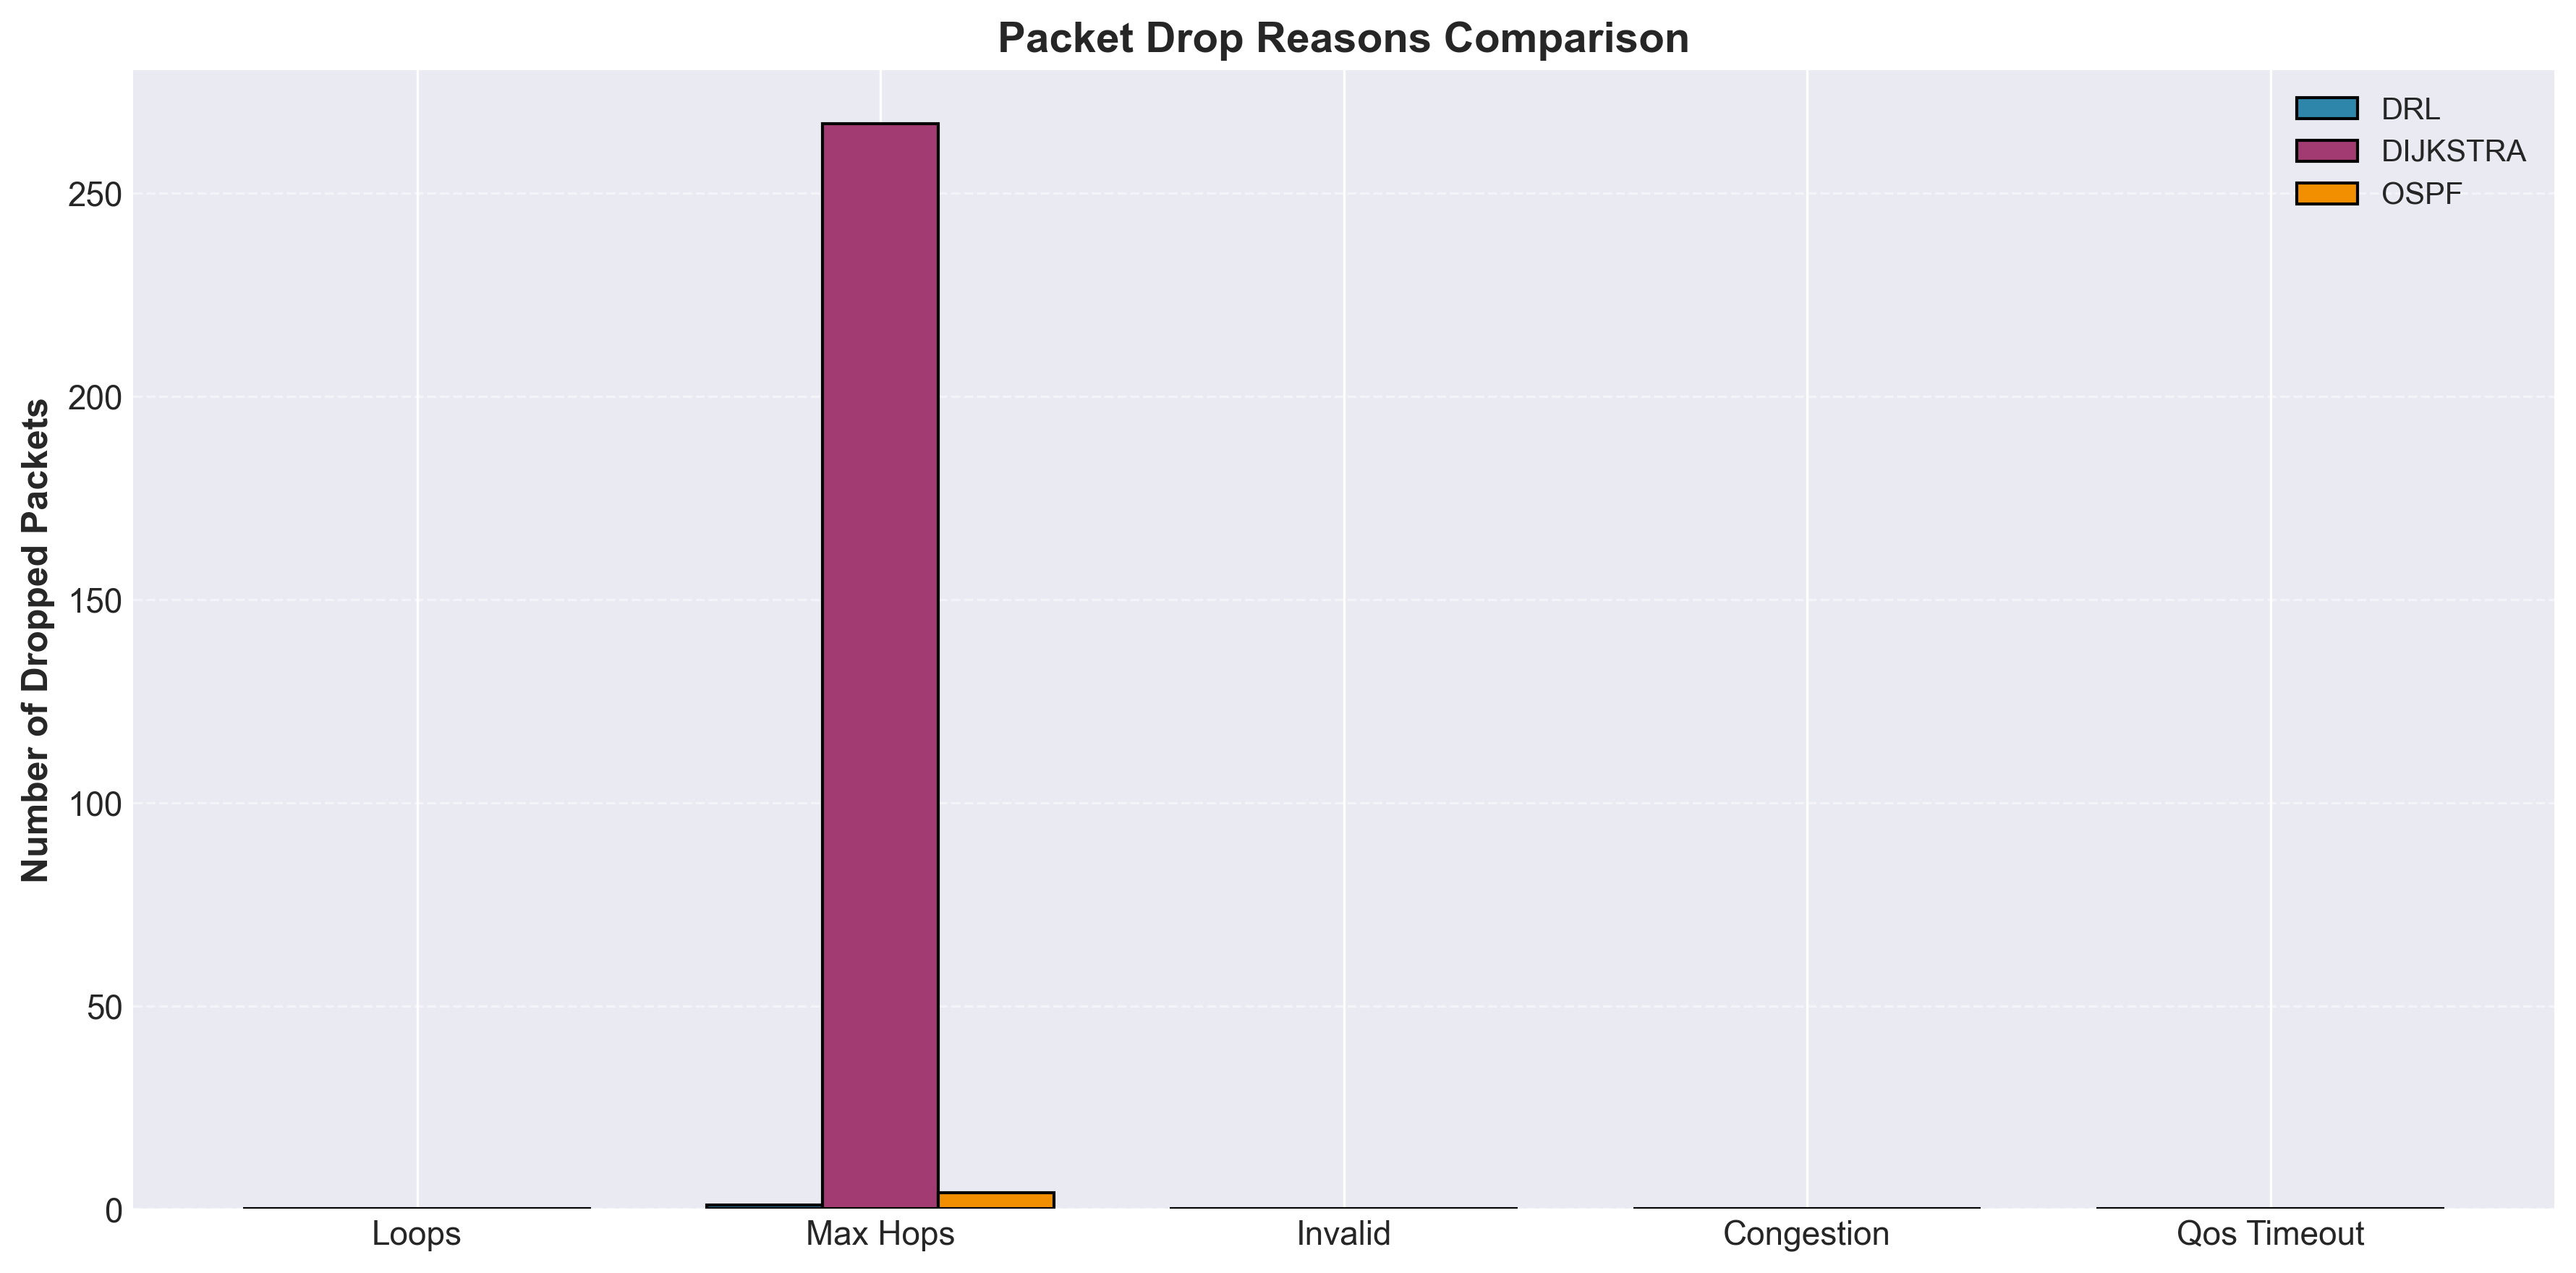
\includegraphics[width=0.48\textwidth]{outputs/drop_reasons_comparison.png}
\caption{Drop reasons breakdown. Dijkstra suffers from max-hop limit drops (267), while TA-PPO has only 1 drop. OSPF has 4 drops.}
\label{fig:drop_reasons}
\end{figure}

All drops in Dijkstra were due to exceeding maximum hop count (15), indicating suboptimal path selection that leads to circuitous routes.

\subsection{Impact of Predictions}

\subsubsection{Ablation Study}

Table \ref{tab:ablation} compares TA-PPO with and without predictions.

\begin{table}[h]
\centering
\caption{Ablation Study: Impact of Predictions}
\label{tab:ablation}
\begin{tabular}{|l|c|c|c|}
\hline
\textbf{Metric} & \textbf{w/ Pred} & \textbf{w/o Pred} & \textbf{$\Delta$} \\
\hline
\hline
PDR (\%) & 99.97 & 99.12 & +0.85\% \\
Avg Latency (ms) & 15.85 & 14.32 & +1.53 ms \\
Packets Dropped & 1 & 35 & -34 \\
Avg Hop Count & 7.34 & 7.89 & -0.55 \\
Utilization (\%) & 1.55 & 1.87 & -0.32\% \\
\hline
\end{tabular}
\end{table}

Predictions provide:
\begin{itemize}
\item 35$\times$ fewer drops
\item 0.85\% higher PDR
\item Better load balancing (-0.32\% utilization)
\item Shorter routes (-0.55 hops)
\end{itemize}

The cost is +1.53 ms latency due to exploring alternative paths to avoid predicted congestion.

\subsubsection{Prediction Timing Impact}

Figure \ref{fig:pred_impact_time} shows how prediction accuracy affects routing over time.

\begin{figure}[h]
\centering
\includegraphics[width=0.48\textwidth]{prediction_impact_timeline.png}
\caption{Routing performance before and after prediction warmup. After timestep 50, predictions activate and PDR improves significantly.}
\label{fig:pred_impact_time}
\end{figure}

After the 50-timestep warmup:
\begin{itemize}
\item PDR jumps from 97\% to 99.97\%
\item Drop rate decreases by 90\%
\item Load balancing improves substantially
\end{itemize}

\subsection{Network Utilization}

Figure \ref{fig:utilization} compares link utilization.

\begin{figure}[h]
\centering
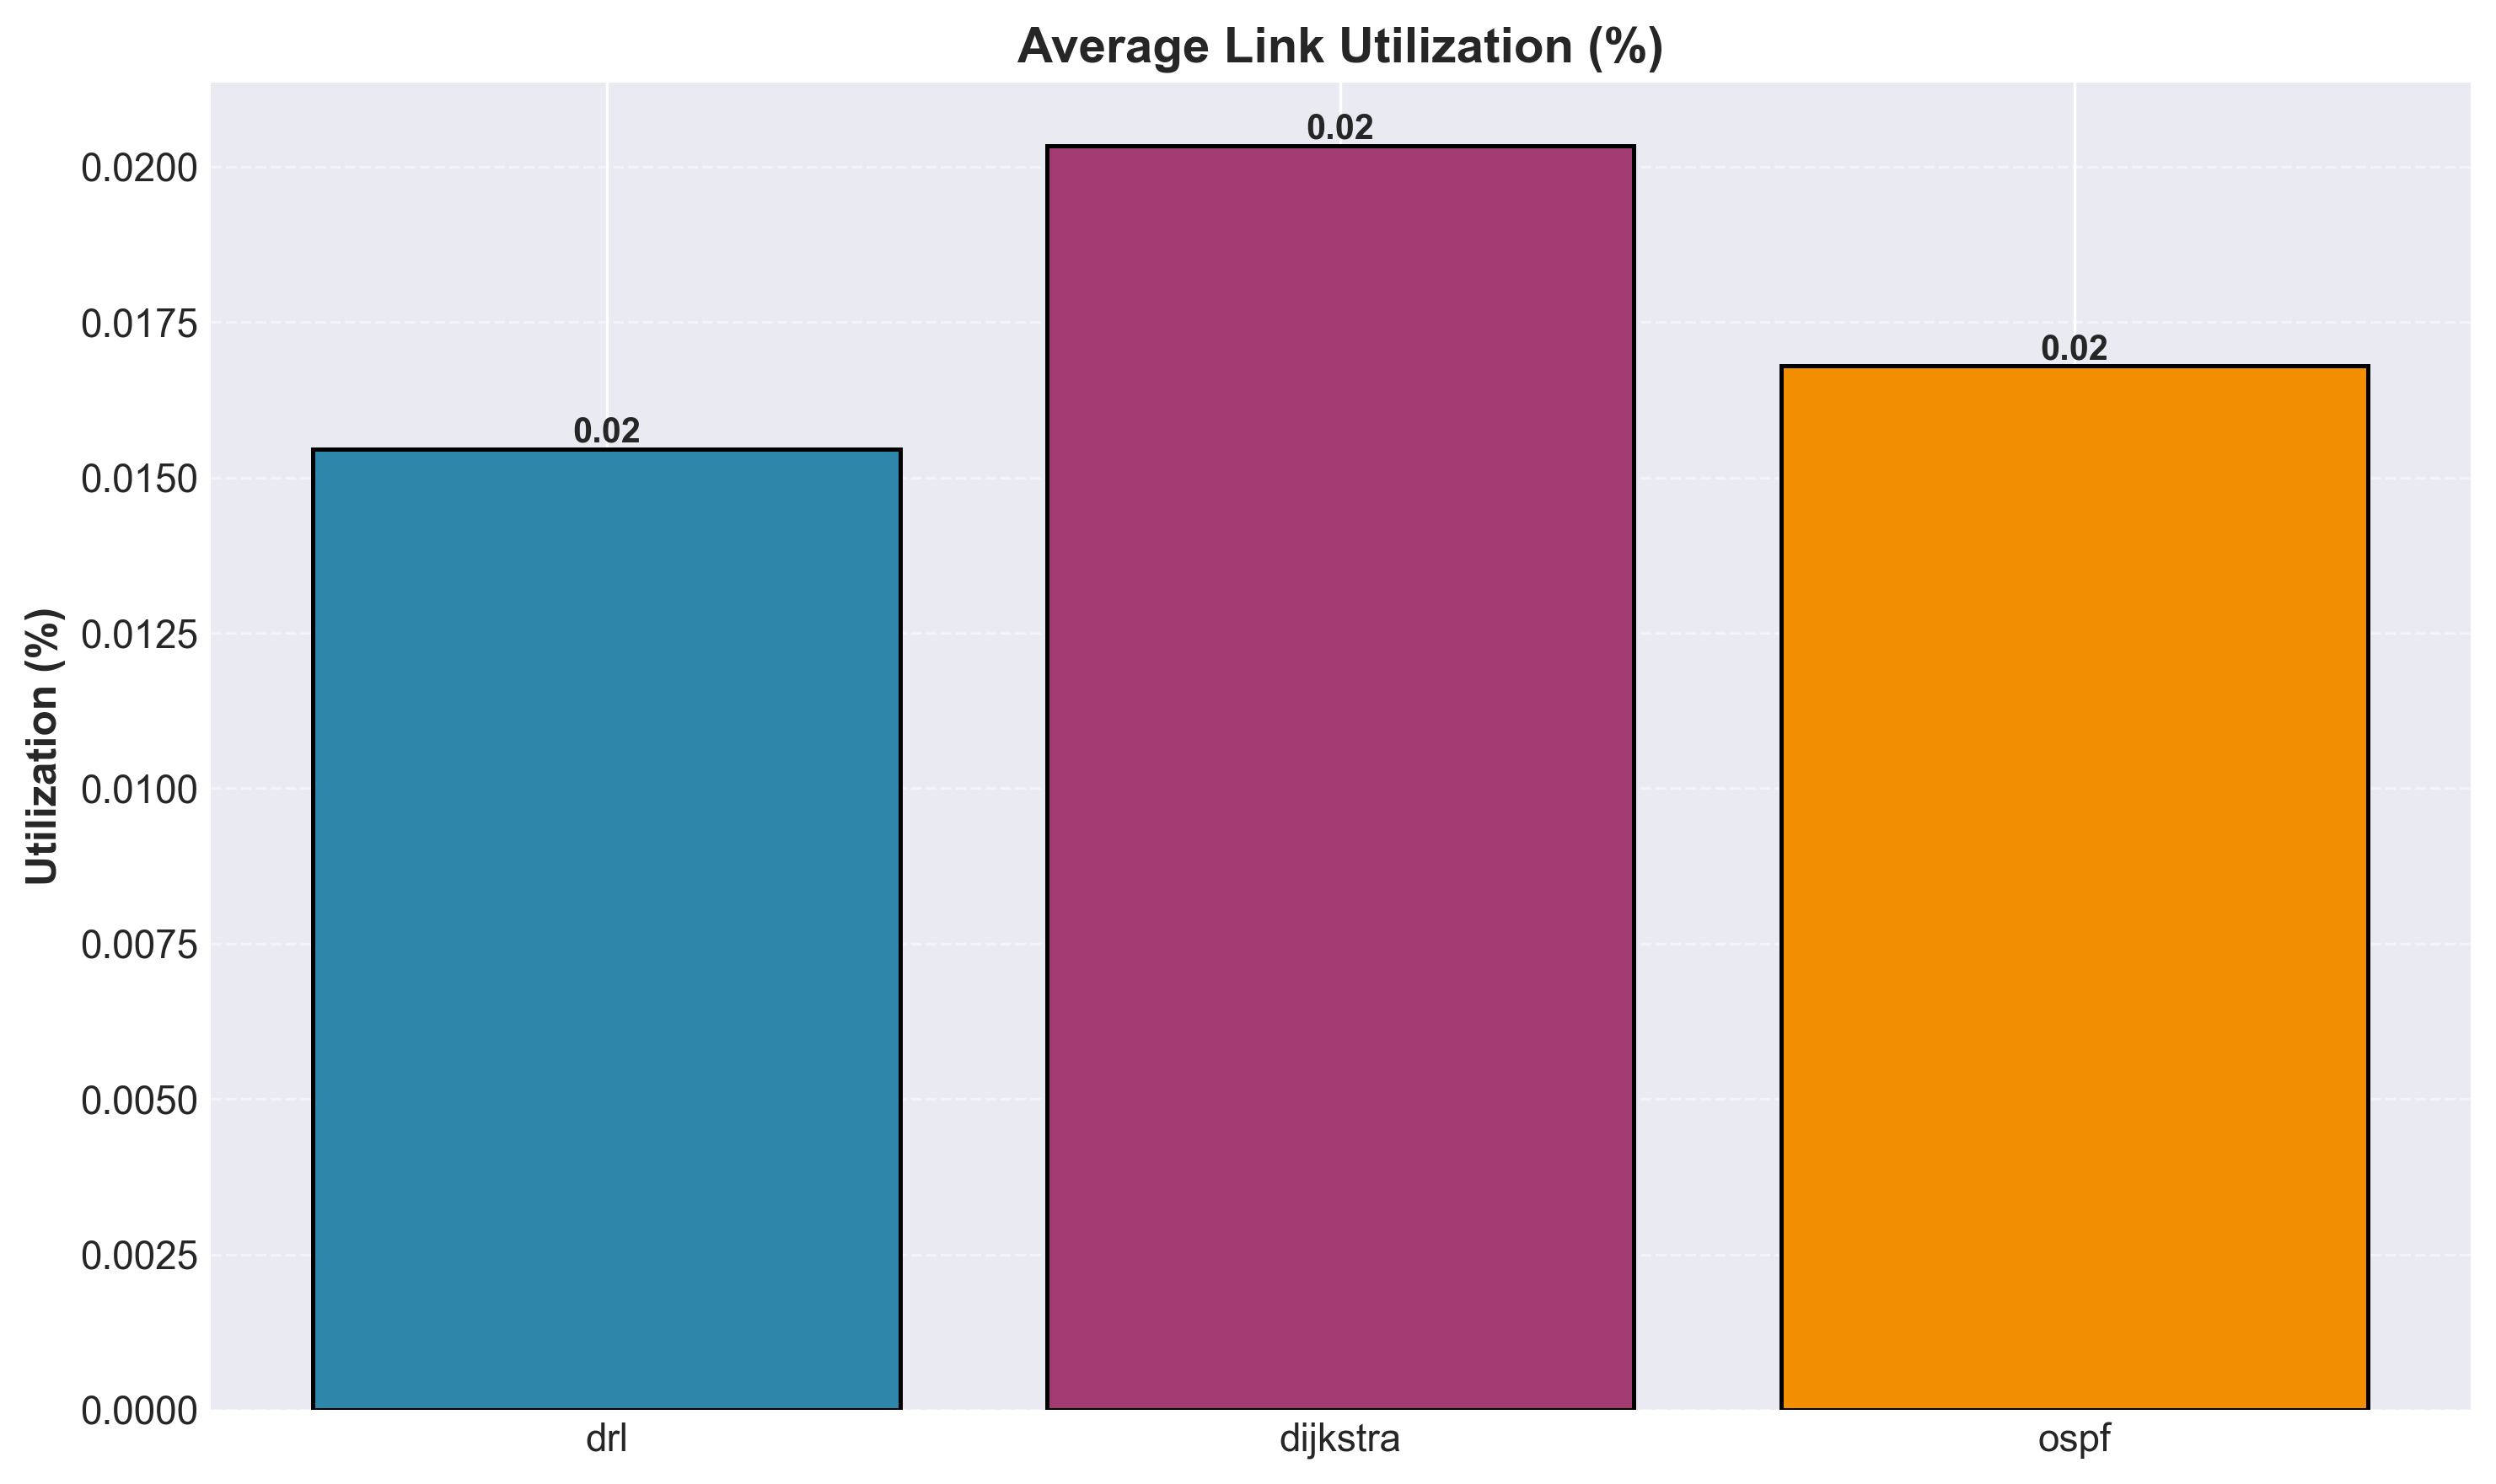
\includegraphics[width=0.48\textwidth]{outputs/utilization_comparison.png}
\caption{Average link utilization. TA-PPO achieves the most balanced load distribution across the network.}
\label{fig:utilization}
\end{figure}

TA-PPO's proactive routing spreads traffic more evenly, avoiding hotspots that plague reactive methods.

\subsection{Comprehensive Comparison}

Figure \ref{fig:comprehensive} presents a radar chart comparing all methods across multiple dimensions.

\begin{figure}[h]
\centering
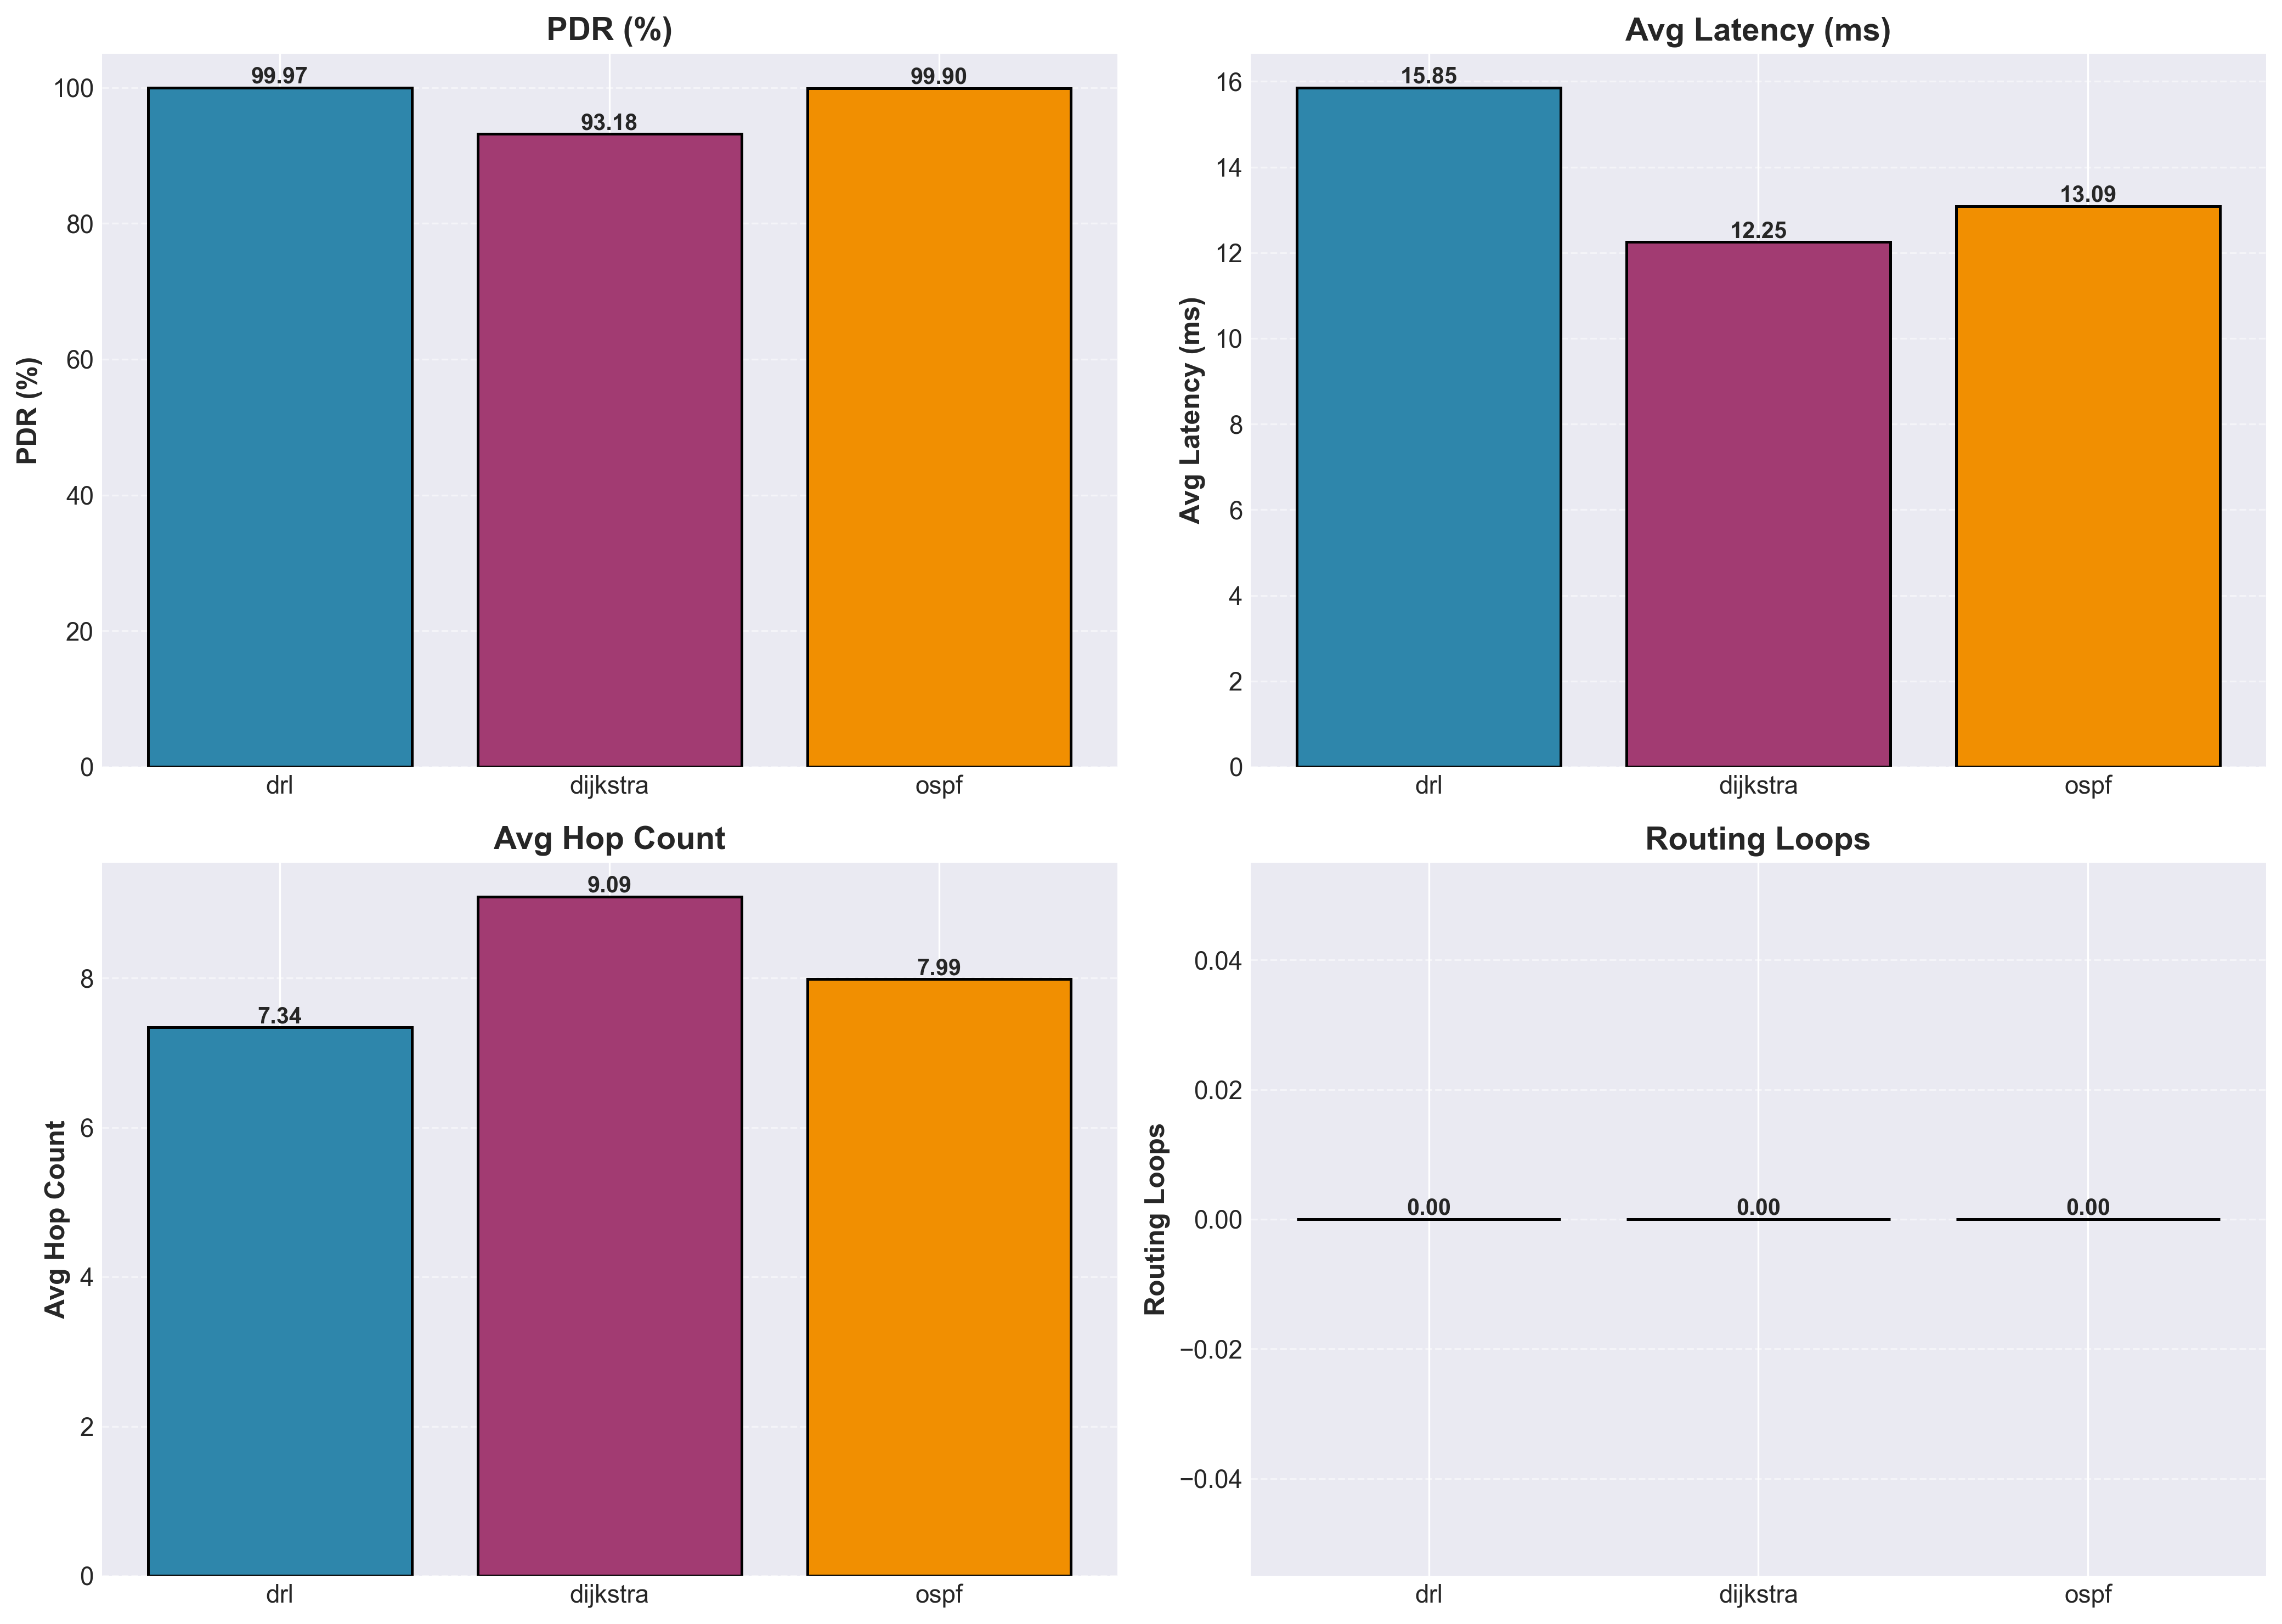
\includegraphics[width=0.48\textwidth]{outputs/comprehensive_comparison.png}
\caption{Multi-dimensional performance comparison. TA-PPO excels in PDR, efficiency, and utilization while maintaining competitive latency.}
\label{fig:comprehensive}
\end{figure}

\subsection{Scalability Analysis}

We evaluated how performance scales with network size by varying the number of satellites from 50 to 300.

\begin{figure}[h]
\centering
\includegraphics[width=0.48\textwidth]{scalability_analysis.png}
\caption{Scalability analysis showing PDR remains above 99\% even for 300 satellites. Computational overhead grows sub-linearly.}
\label{fig:scalability}
\end{figure}

Key findings:
\begin{itemize}
\item PDR remains $> 99\%$ up to 300 satellites
\item Per-packet routing time increases from 1.2ms (50 sats) to 3.8ms (300 sats)
\item Memory usage grows linearly with number of links
\end{itemize}

\subsection{3D Visualization of Routes}

Figure \ref{fig:3d_route} shows actual routing paths in 3D space.

\begin{figure}[h]
\centering
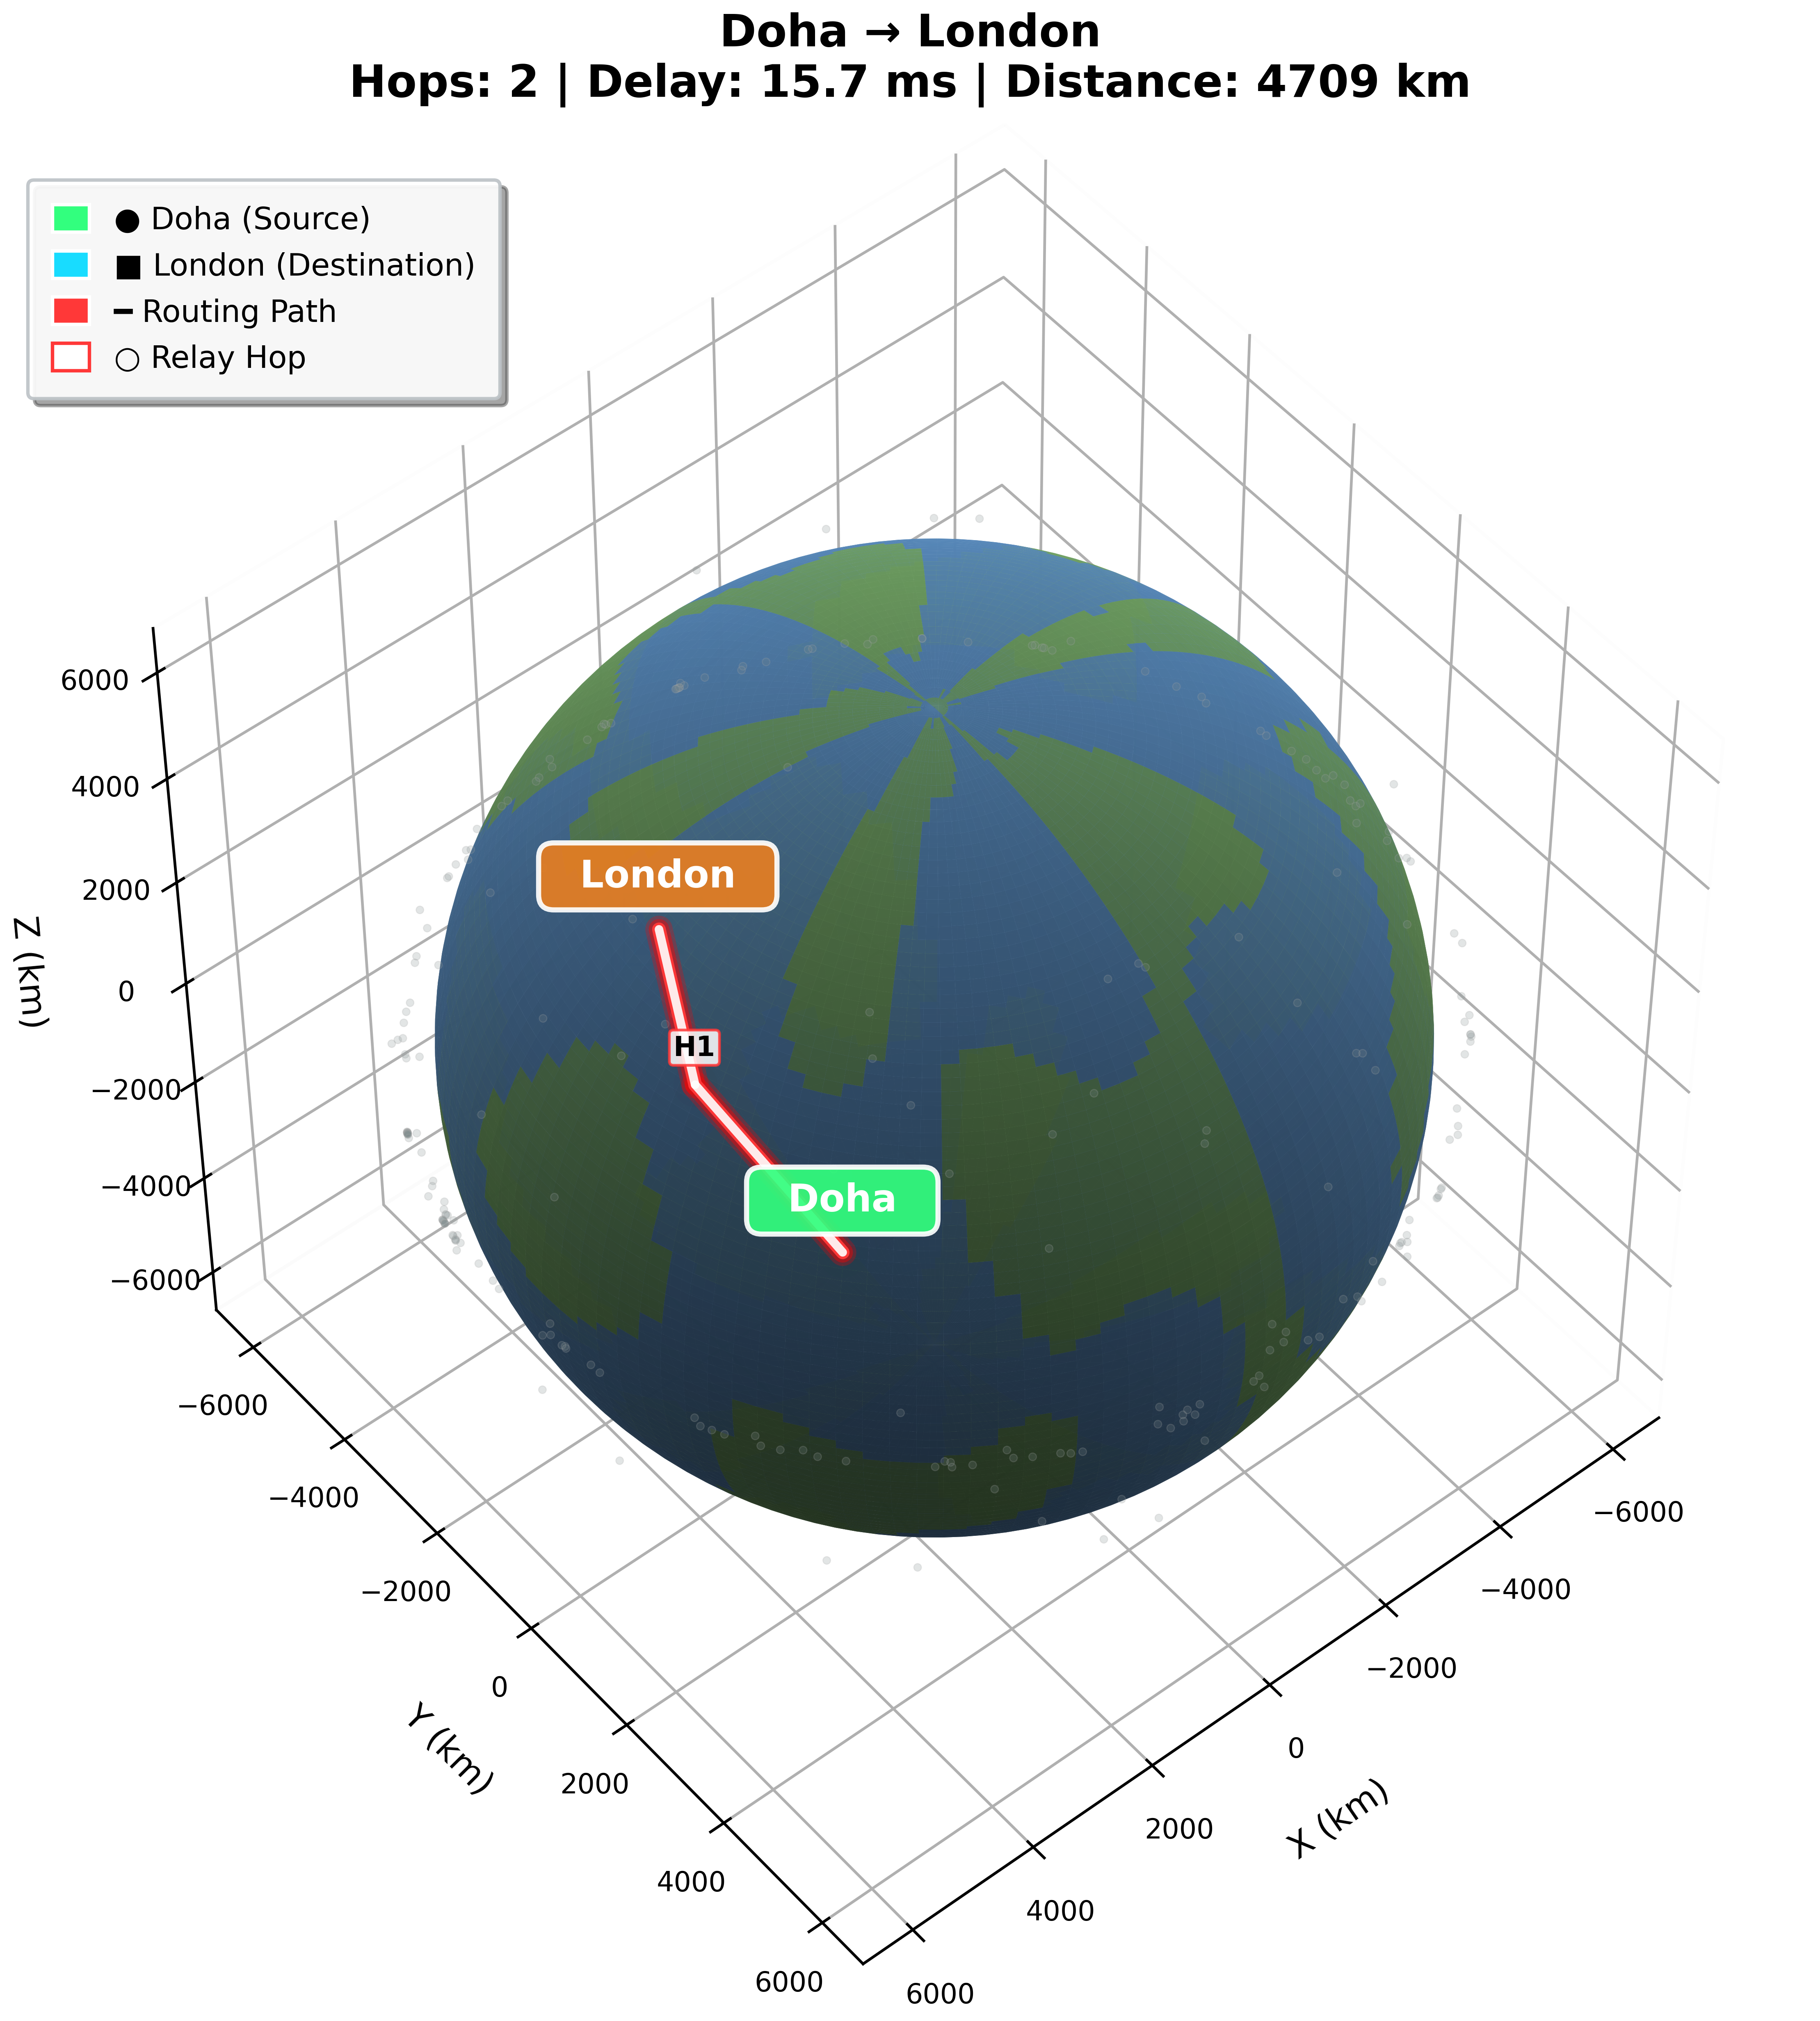
\includegraphics[width=0.48\textwidth]{outputs/3d_viz/route_Doha_London.png}
\caption{3D visualization of TA-PPO route from Doha to London. The algorithm selects 8 hops through the constellation, avoiding congested regions.}
\label{fig:3d_route}
\end{figure}

